\documentclass{report}

\usepackage[utf8]{inputenc}
\usepackage[english]{babel}
\usepackage[babel=true,final]{microtype}
\usepackage{listings}
\usepackage{url}
\usepackage[linktocpage]{hyperref}
\usepackage{geometry}
\usepackage{tikz}
\usetikzlibrary{shapes,snakes,arrows,calc,decorations,shadows}

% listings
\lstset{
	%framerule=1pt,
	frame=lines,
	basicstyle=\small,
%	commentstyle=\rm\color{color1!50!black},
}

% margins
\geometry{hmargin=3.4cm,vmargin=3.2cm}

\newcommand{\ie}{{\it i.e.}~}
\newcommand{\eg}{{\it e.g.}~}
\newcommand{\cf}{{\it c.f.}~}
\newcommand{\etal}{~{\it et al.}}
\newcommand{\etc}{{\it etc.}}

\newcommand{\rchap}[1]{Chapter~\ref{ch:#1}}
\newcommand{\rsec}[1]{Section~\ref{sec:#1}}
\newcommand{\rssec}[1]{Sub-section~\ref{ssec:#1}}
\newcommand{\rfig}[1]{Figure~\ref{fig:#1}}
\newcommand{\rtab}[1]{Table~\ref{tab:#1}}

\newenvironment{example}{
\begin{minipage}{0.7\textwidth}
{\em Example:}
}{
\end{minipage}
\newline
}

\sloppy

\begin{document}

\begin{titlepage}

% \begin{center}
% \large
% Alex Negrea \hspace{2cm} Simon Duquennoy
% \end{center}

~

\vspace{6cm}

\begin{center}

\includegraphics{smewsLogo}
\end{center}

\begin{center}
\LARGE
{\em Smart \& Mobile Embedded Web Server}

User Guide
\end{center}

\vfill

\begin{center}
\em
Last revised: \today
\end{center}

\end{titlepage}

\tableofcontents
 
\chapter{Introduction}

\section{What is Smews?}

Smews stands for \emph{Smart \& Mobile Embedded Web Server}. This research prototype is designed for hardware-constrained devices like smart cards, sensor boards and other small devices. It is a stand-alone software, working without any underlaying OS. It acts as the OS by itself, dedicated to the support of Web applications. Its kernel includes device drivers, TCP/IP stack, Web server and Web applications container. It is based on a event-driven architecture and its implementation is full of cross-layer optimizations.

Web applications are pre-processed, compiled, linked with Smews then embedded in a device. Web applications are made of static and dynamic contents. Static contents are simple files; dynamic contents are linked to server-side code. During the pre-processing phase, plenty of optimizations are made on Web contents (pre-calculation of protocol headers, checksums, parsing. automatons). Smews supports Comet (server-pushed data) and provides an advanced typing of dynamic Web contents (persistent, idempotent and volatile contents). The post request processing is also implemented.

\section{About this guide}

This document contains the necessary information to get started with Smews, understand its philosophy and master its usage. It should be read by both users willing to use Smews and developers wanting to be introduced to Smews functionalities.

\rchap{gettingstarted} contains information about Smews compilation, installation and execution, giving detailed features descriptions and concrete examples. \rchap{creatingapp} explains how to build your own Web application for Smews.

\chapter{Getting Started}
\label{ch:gettingstarted}

\section{Preparing your environment}

You can download the latest Smews release from its Github repository \url{http://github.com/2xs/smews}

In order to work with Smews, you will need:
\begin{itemize}
  \item a valid C compilation environment, depending on your platform the target:
	\begin{itemize}
	  \item \emph{for target MicaZ and Funcard7} you will need: \verb+gcc-avr+  (4.3 or above) and \verb+avr-libc+ packages;
	  \item \emph{for target MSP430} you will need the following packages: \verb+binutils-msp430+, \verb+msp430-libc+, \verb+gcc-msp430+. These packages can be found in \verb+deb+ \url{http://wyper.ca/debian/} \verb+i686+ repository;
	  \item \emph{for target GBA} you will need: DevKitAdvance (\url{http://devkitadv.sourceforge.net/});
	  \item \emph{for target MBED} you will need: \verb+arm-none-eabi-gcc+. This version of gcc can be built using the script available at (\url{https://github.com/esden/summon-arm-toolchain}). For the ethernet version of the mbed port, you will also need rflpc library. This library can be automatically downloaded and compiled by running the \verb!summon-rflpc! script in the \verb!targets/mbed_ethernet! folder.
	\end{itemize}
  \item Python version 2.5 or above;
  \item SCons version 0.96 or above.
\end{itemize}

The Smews compilation process is based on SCons and Python. It has been tested on Linux, Windows (using MinGW) and Mac OS.

\section{What's in the package?}

In the Smews package you can find the following directories and files:
\begin{itemize}
\item \verb+SConstruct, SConscript+
-- Smews general SCons files;
\item \verb+apps/+
-- examples of Web applications to be served by Smews;
\item \verb+core/+
-- Smews kernel C source code (portable files);
\item \verb+panManager/+
-- Personal Area Network manager (setting device-computer link);
\item \verb+tools/+
-- Python preprocessing tools (used by the SCons compilation chain);
\item \verb+targets/+
-- Smews ports to different devices.
\end{itemize}

Every port is made of a directory in \verb+targets/+. Target-dependent code is located in \verb+targets/$target/drivers+. The \verb+targets/$target/SConscript+ file defines target-specific compilation instructions. The \verb+targets/$target/install+ script is in charge of installing Smews on the target device. The following lines describe all existing Smews ports.
%$

\paragraph{WSN430}

The WSN430 sensor board is based on a 16-bits msp430 processor at 8 MHz. Communications are done over a serial line by using the SLIP protocol.

\paragraph{MicaZ}

The MicaZ sensor board is based on a 8-bits AVR processor at 8 MHz. Communications are done over a serial line by using the SLIP protocol.

\paragraph{Funcard7}

The Funcard7 smart card is based on a 8-bits AVR processor at 4 MHz. Communications are done over a serial line using a custom "IP over APDU" protocol.

\paragraph{GBA}

The Game Boy Advance is based on a 32-bits Arm7 processor at 16 Mhz. Communications are done over a serial line by using the SLIP protocol.

\paragraph{MBED}

The MBED platform is a popular prototyping board based on the LPC1768 SoC by NXP. It includes an ARM Cortex-M3 32bits processor at 100Mhz as well as an ethernet mac 100Mbps full duplex. Smews as been ported to this platform using SLIP and ethernet. Note that before compiling for the \verb+mbed_ethernet+ target, you have to run the \verb+targets/mbed_ethernet/summon-rflpc+ script. In order to make the port work in IPv6, you should add the \verb!icmpv6! application that will handle neighbor solicitation packets.

\paragraph{Linux}

This target has been written for debug and development purposes. It allows to execute Smews as a linux process, communicating {\it via} the TUN virtual interface.

\paragraph{Skeleton}

This target is an empty one. It is a starting point for someone wanting to port Smews to a new device.

\section{Compiling Smews}
\label{sec:compile}

Smews uses SCons for building which allows to design complex build mechanism and dependencies. The multiple pre-processing steps help Smews to be more efficient in terms of memory consumption and processing speed.

\subsection{Short description}

When building Smews you can specify multiple targets and Web applications to be embedded with it. For example to build Smews for a destination target A and B (directories in \verb+targets/+) and embed in it Web Applications X and Y (directories in \verb+apps/+) you can type:

\begin{verbatim}
$ scons target=A,B apps=X,Y
\end{verbatim}

Files are compiled in the \verb+bin/$target+ directory. This contains the Smews executable file. It also contains a \verb+libsmews.a+ file, allowing to embed Smews in other software (see \verb+core/main.c+ provided as a sample main C code linked with the library \verb+libsmews.a+).

To clean built files type:
\begin{verbatim}
$ scons -c
\end{verbatim}

For a complete description of available arguments, type:
\begin{verbatim}
$ scons -h
\end{verbatim}

\subsection{Exhaustive description}

The Smews compilation chain has many arguments enabling different options. The only necessary argument for a build is \verb+target+. All other arguments are optional and have a default value. \rtab{sconsargs} synthesizes the list of available arguments. We give here a precise description of every argument.

\begin{table}
    \fbox{
      \colorbox{black!10}{
		\begin{minipage}{1\textwidth}
{\tt target=targetA,targetB,...}
\par\hspace{0.1\textwidth} targets on which to compile Smews

{\tt apps=[urlA:]appA,[urlB:]appB,...}
\par\hspace{0.1\textwidth} applications to be embedded with Smews

{\tt ipaddr=ip}
\par\hspace{0.1\textwidth} set the Smews IP address

{\tt debug=true|false}
\par\hspace{0.1\textwidth} enable or disable debug mode

{\tt gzip=true|false}
\par\hspace{0.1\textwidth} enable or disable static Web contents compression

{\tt chuncksNbits=number}
\par\hspace{0.1\textwidth} size of the chuncks used for pre-calculated checksums

{\tt endian=little|big}
\par\hspace{0.1\textwidth} data endianness

{\tt disable=[arguments|comet|retransmit|post|gpip]+}
\par\hspace{0.1\textwidth} disable internal functionalities

		\end{minipage}
      }
   } 
\caption{Smews compilation options}
\label{tab:sconsargs}
\end{table}

\subsubsection{Option {\tt target=targetA,targetB,...}}

Set the target(s) on which Smews is going to be compiled. Example:
\begin{verbatim}
$ scons target=linux,WSN430
\end{verbatim}

\subsubsection{Option {\tt apps=[urlA:]appA,[urlB:]appB,...}}

Specifies the set of Web applications that will be linked and embedded with Smews. An application is a directory or sub-directory in the \verb+apps+ directory. Every application is made of simple files (static Web contents) and/or C files (dynamic Web contents). Contents are separated by comma and the name of the content can be preceded by a replacement URL. Default value: \verb+apps=:welcome+. Example:
\begin{verbatim}
$ scons target=linux apps=contactsBook,mycalendar:calendar,:welcome
\end{verbatim}

Resources extracted from directories \verb+contactsBook+, \verb+calendar+ and \verb+smews+ will be respectively accessible at the following URLs:

\url{http://$smewsip/contactsBook}

\url{http://$smewsip/mycalendar}

\url{http://$smewsip/}
%$

\subsubsection{Option {\tt ipaddr=ip}}

Set the Smews IP address. Can be either a IPv4 or IPv6 address. Examples:
\begin{verbatim}
$ scons target=linux apps=:welcome ipaddr=192.168.1.2
$ scons target=linux apps=:welcome ipaddr=2001::2
\end{verbatim}

\subsubsection{Option {\tt debug=true|false}}

Allows to compile Smews in debug mode, without any optimization (\verb+gcc -g -O0+ options). Default value: \verb+debug=false+. Example:
\begin{verbatim}
$ scons target=linux apps=:welcome debug=true
\end{verbatim}

\subsubsection{Option {\tt gzip=true|false}}

Allows to compress static files at compile time. This reduces the target footprint, but the client browser must be able to unpack the content. Default value: \verb+gzip=true+. Example:
\begin{verbatim}
$ scons target=linux apps=:welcome gzip=false
\end{verbatim}

\subsubsection{Option {\tt chuncksNbits=number}}

In Smews, the checksums of static files are pre-calculated on chunks of data at compile time. The size of the chunks is computed as \verb+1<<chuncksNbits+. The size of outgoing segments is limitated by this size since it has to be multiple of it. Default value: \verb+chuncksNbits=5+.
\begin{verbatim}
$ scons target=linux apps=:welcome chunckNbits=5
\end{verbatim}

\subsubsection{Option {\tt endian=little|big}}

Forces data little or big endianness. Default value depends on the target (\verb+ENDIANNESS+ C macro defined in the \verb+target/$target/target.h+ file). Example:
\begin{verbatim}
$ scons target=linux apps=:welcome endian=little
\end{verbatim}

\subsubsection{Option {\tt disable=[arguments|comet|retransmit]+}}

Allows to disable some internal functionalities, making the binary smaller and the execution faster:
\begin{itemize}
\item \texttt{arguments} -- URL arguments parsing will be removed from the source code;
\item \texttt{comet} -- removes comet support in the binary, which disallows the server to push data to the client;
\item \texttt{retransmit} -- disable TCP packets retransmission in case of lost segments. The generated web server will not be fully compliant with the TCP RFC.
\end{itemize}

Example:
\begin{verbatim}
$ scons target=linux apps=:welcome disable=comet,arguments
\end{verbatim}

\section{Installing Smews}
\label{sec:install}

Once Smews has been compiled, it can be embedded in the target device. This step can be done by executing the \verb+target/$target/install+ script.
%$

Then, the panManager has to be launched. It enables the communication between a computer and a device, managing the link-layer protocol. When launching the panManager, two arguments are mandatory:

\begin{description}
\item[Plugin] The first argument is the plugin, implementing the desired link-layer protocol. Currently, the two existing plugins are SLIP (Serial Line IP) and APDUIP (APDU supporting IP). For SLIP, you can specify the serial device using the -p option (/dev/ttyS0 by default). 
\item[IP configuration] The second argument is used to configure the computer routing table. It describes an IP address and a mask size by using the "slash" notation. The panManager supports either IPv4 and IPv6 addresses.
\end{description}

Example: configuring a SLIP link with local address 192.168.1.1 and a 24-bits mask:
\begin{verbatim}
$ panManager slip 192.168.1.1/24
\end{verbatim}

Example: configuring a APDUIP link with local address 2001::1 and a 126-bits mask:
\begin{verbatim}
$ panManager apduip 2001::1/126
\end{verbatim}

After this step, you can reach Smews at its IP address by using any HTTP/1.1 compliant Web client.

\section{Simple example, step by step}

We synthesize the previous sections by giving a complete example where we compile, install and access Smews on a WSN430 sensor board. All commands are given from the main Smews directory.

Compilation, embedding the welcome page and sensor application, with IPv4 address 192.168.1.2:
\begin{verbatim}
$ scons target=WSN430 apps=:welcome,sensor ipaddr=192.168.1.2
\end{verbatim}

Installation, \ie{} copy of the code in the EEPROM of the WSN430 board (as root):
\begin{verbatim}
$ ./targets/WSN430/install
\end{verbatim}

PanManager configuration (as root, in panManager folder):
\begin{verbatim}
$ bin/panManager slip 192.168.1.1/24
\end{verbatim}

\chapter{Creating your own Web Application}
\label{ch:creatingapp}

Web applications are made of static (files) and dynamic (generated by the server at runtime) contents. Applications are identified by subdirectories of the \texttt{apps/} directory. The \texttt{apps/examples} contains application examples using various features of Smews. A folder identifies a particular Web Application or a set of Web applications which will be embedded in the web server (see \rsec{compile} for more details). Every application is made of a set of files, of various types :
\begin{description}
\item[.c and .h files] C and H files are used to embed server-side code, compiled and linked with Smews;
\item[.c files with XML] C files containing specific XML meta-data (as c comment) are associated to Web resources, \ie{} they are in charge of generating dynamic Web contents in response to client requests;
\item[other files] Other files are considered as static. They will be embedded and served by Smews "as is";
\item[.c.embed files] The .embed extension is automatically removed. This allows to serve a C file as a static content.
\end{description}

\section{Static Content}

When embedding static file in Smews, the HTTP content-type field is automatically inferred from the file extension (the mappings list is contained in the file \texttt{tools/mimeRessources}). Furthermore, many optimizations occur off-line, including HTTP header and TCP checksums pre-calculation. As an example, create a new file containing the following code and save it in \texttt{apps/helloWorld/hello.html}:

\lstset{language=html}
\begin{lstlisting}
<html>
    <head>
        <title>Hello World!</title>
    </head>
    <body>
        Hello World!
    </body>
</html>
\end{lstlisting}

Compile Smews setting the target to \verb+linux+ and the content to be embedded \verb+helloWorld+ as below:
\begin{verbatim}
$ scons target=linux apps=helloWorld ipaddr=192.168.1.2
\end{verbatim}

Then run the ELF file from the \texttt{/bin/linux} directory. You can now access the server at \verb+http://192.168.1.2/helloWorld/hello.html+. Keep in mind that the linux target is a particular case where Smews binary file is a process, that is why it can be launched directly. If tested on different target, refer to the instructions in \rsec{install}.

\section{Dynamic Content}

Smews can serve content generated by native code, which we will refer to as \textit{Dynamic Content}. Any C file containing XML specific code (as C comment) will considered as a Web resource and associated to an URL. The XML meta-data are interpreted in the pre-processing phase, thus generating some C code. We describe here the role of the XML markers available (a detailed list is given in \rtab{appsxml}, page \pageref{tab:appsxml}).

\subsection{Defining handlers}

Web applications are scheduled by Smews {\it via} a pre-defined set of handler functions (a detailed list is given in \rtab{appscallbacks}, page \pageref{tab:appscallbacks}):
\begin{itemize}
\item \verb+init+ -- function executed during Smews initialization;
\item \verb+initGet+ -- function executed when a Get request is received ;
\item \verb+doGet+ -- function used to generate the HTTP response.
\end{itemize}

The XML meta-data allows to associate C functions to these handlers. As an example, create a new file containing the following code and save it in \texttt{apps/helloWorld2/hello.c}:
\lstset{language=C}
\begin{lstlisting}
/*
<generator>
	<handlers doGet="do_hello"/>
</generator>
*/

/* simple contents generator */
static char do_hello(struct args_t *args) {
    out_str("Generated Hello World!");
    return 1;
}
\end{lstlisting}

You can now access the server at \verb+http://192.168.1.2/helloWorld2/hello+. On the server side, the \verb+doHello+ function will be called by Smews when a the response to the client request has to be generated. The \verb+out_str+ function outputs a string as the HTTP response (a detailed list of the functions provided by Smews to Web applications is given in \rtab{appssyscalls}, page \pageref{tab:appssyscalls}).

\subsection{Parsing URL arguments}

Smews allows to parse URL arguments before calling the \verb+doGet+ handler. This parsing is processed in the kernel, so it is quite efficient and requires few memory. The format of the arguments are defined statically. At compile-time, a parsing automaton is generated for every dynamic Web resources, allowing an efficient arguments parsing. Here is an example where URL arguments are parsed then sent as an HTTP response:

\lstset{language=C}
\begin{lstlisting}
/*
<generator>
    <handlers doGet="output_args"/>
    <args>
        <arg name="i1" type="uint8" />
        <arg name="s" type="str" size="6" />
        <arg name="i2" type="uint16" />
    </args>
</generator>
*/

static char output_args(struct args_t *args) {
    if(args) {
        out_str("first int : ");
        out_uint(args->i1);
        out_str("\nstr : ");
        out_str(args->s);
        out_str("\nsecond int : ");
        out_uint(args->i2);
    } else {
        out_str("no args");
    }
    return 1;
}
\end{lstlisting}

The \verb+args+ parameter points to the values of the arguments that have been parsed by Smews. Every URL argument is directly accessible as a field of the \verb+struct args_t+ structure, with the name that has been described in the XML meta-data. The \verb+out_uint+ function is used to output an integer.

\subsection{Persistence of the generated data}

Smews provides an advanced typing of dynamic contents. The internal behavior of the Smews TCP/IP stack automatically adapts to this typing, allowing to output many simultaneous segments while keeping memory consumption as low as possible. Three types of persistence have been defined:
\begin{description}
\item[volatile] -- means that the content generated will not be stored in memory and will be regenerated in case of TCP NACK;
\item[idempotent] -- means that the function will return the same value no matter when you might call it (it is deterministic and has no side-effect). In the current implementation, idempotent data are managed is the same manner than volatile data;
\item[persistent] (default option) -- means that the output will be kept in memory and will be delivered from there in case of NACK.
\end{description}

Here is an example of a volatile Hello World. In case of TCP loss, the HTTP response may generated several times by multiple calls of the \verb+doGet+ function:
\lstset{language=C}
\begin{lstlisting}
/*
<generator>
    <handlers doGet="do_hello_v"/>
    <properties persistence="volatile"/>
</generator>
*/

/* possible persitence are persistent (by default), idempotent and volatile */
static char do_hello_v(struct args_t *args) {
    out_str("Volatile Hello World!");
    return 1;
}
\end{lstlisting}

\subsection{Interaction mode}

Smews also supports Web push, often called \emph{Comet}. In Smews, Comet is implemented {\it via} channels. A channel is a way of sending data asynchronously by pushing it from server to a set of registered clients. To see how can you accomplish this take a look at the next example:
\lstset{language=C}
\begin{lstlisting}
/*
<generator>
    <handlers doGet="waitknock"/>
    <properties interaction="alert" channel="knockknock"/>
</generator>
*/

/* launched when knockknock is triggered */
static char waitknock(struct args_t *args) {
    out_str("somebody knocked");
    return 1;
}
\end{lstlisting}

The above example set the interaction tag to \verb+alert+, and defines a channel named \verb+knockknock+. In alert mode, HTTP client requests are not answered as soon as they are received. Instead, they are simply registered as listening to the \verb+knockknock+ channel. The request is pending until an event occurs.

Let's create a second Web resource as follows: 
\lstset{language=C}
\begin{lstlisting}
/*
<generator>
    <handlers doGet="triggerknock"/>
</generator>
*/

/* triggers the knockknock comet channel */
static char triggerknock(struct args_t *args) {
    server_push(&knockknock);
    return 1;
}

\end{lstlisting}

When a request targets this second resource, the \verb+triggerknock+ function is called. It triggers the \verb+knockknock+ channel. At this time, the \verb+waitknock+ is called, thus generating a HTTP response containing the string "somebody knocked". This response will be sent to all registered clients.

Three interaction mode are supported by Smews:
\begin{description}
\item[rest] This is the default mode, corresponding to the classical HTTP request/response scheme;
\item[alert] Incoming requests are pending, they will be answered when the associated channel is triggered;
\item[stream] Incoming requests are pending. Every time the associated channel is triggered, a chunk of HTTP response is generated and sent to all listening clients. The HTTP response is possibly never-ending.
\end{description}

\subsection{Timers}

Any Web application in Smews can use timers in order to execute a function at a given interval. As an example, this feature may be used in a sensor board to periodically check the current temperature. When the sampled value reaches a threshold, a HTTP chunck containing the data is sent to all registered clients {\it via} the stream interaction modes:
\lstset{language=C}
\begin{lstlisting}
/*
<generator>
        <handlers init="init_adc_timer"
	      initGet="set_threshold" doGet="send_temperature"/>
        <properties persistence="volatile"
                interaction="stream" channel="tempAlert" />
        <args> <arg name="threshold" type="uint16" /> </args>
</generator>
*/

static uint16_t threshold = 512;
static uint16_t curr_sample;

/* timer callback, checking the temperature */
static void check_temp() {
        uint16_t tmp_result = get_adc_val(ADC_TEMP);
        if(tmp_result >= threshold) {
	      curr_sample = tmp_result;
	      trigger_channel(&tempAlert);
        }
}

/* initializes ADC and timer */
static char init_adc_timer(void) {
        return init_adc(ADC_TEMP) && set_timer(&check_temp, 200);
}

/* called when a get request is received. initializes the threshold */
static char set_thresholds(struct args_t *args) {
        if(args != NULL) {
	      threshold = args->threshold;
	      return 1;
        } else return 0;
}

/* called to generate the HTTP response */
static char send_temperature(struct args_t *args) {
        out_uint(curr_sample);
        return 1;
}
\end{lstlisting}

The \verb+init_adc_timer+ function is called during Smews initialization. It associates the \verb+check_temp+ function to a timer, asking Smews to execute it every 200~ms. It also initializes the ADC (allowing to sample the temperature). When a client request is received, the \verb+set_thresholds+ function is called, thus setting the current threshold. The periodic timer executed every 200~ms compares the current temperature to this threshold. If needed, it triggers the channel, thus sending the current time to every registered clients. This produces an infinite HTTP response: the Web browser receives new data whenever the threshold is reached.

\section{Post request processing}
Smews supports post request processing, which are used to send lots of data. Smews considers two types of data : forms and files. The C files containing XML specific code (as C comment) like to generate dynamic content (see 3.2 section).    

\subsection{Form}
Example of a HTML form :

\begin{lstlisting}
<form action="post_test_1" method=post>
	<label>int :</label>
	<input type="text" name="i1" id="i1" value="4" />
	<br />
	<label>str :</label>
	<input type="text" name="s" id="s" value="toto" />
	<br />
	<label>int :</label>
	<input type="text" name="i2" id="i2" value="5" />
	<input type=submit value="Submit"/> 
</form>
\end{lstlisting}

Display from a web browser :
\begin{center}
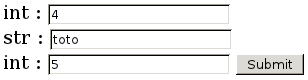
\includegraphics{form}
\end{center}

SMEWS needs doPost function and arguments (like to parse URL arguments, see 3.2.2 section).

\lstset{language=C}
\begin{lstlisting}
/*
<generator>
    <handlers doPost="output_args"/>
    <args>
        <arg name="i1" type="uint8" />
        <arg name="s" type="str" size="6" />
        <arg name="i2" type="uint16" />
    </args>
</generator>
*/

static char output_args(struct args_t *args) {
    if(args) {
        out_str("first int : ");
        out_uint(args->i1);
        out_str("\nstr : ");
        out_str(args->s);
        out_str("\nsecond int : ");
        out_uint(args->i2);
    } else {
        out_str("no args");
    }
    return 1;
}
\end{lstlisting}
The process is similar to get request processing with arguments.

\subsection{Received Post Files}
To send files to the server Smews, use multipart data with HTML. Here are two examples to manage one or more files, with an application that counts all characters of send files.
\newline
\newline
Example of a HTML form to send files :
\begin{lstlisting}
With Single File
<form enctype=multipart/form-data action="app_counter_simple" method=post>
	<input type=file name=filename value="Choose file"/>
	<input type=submit value="Submit"/>
</form>	
<br />
With Several Files
<form enctype=multipart/form-data action="app_counter_multi" method=post>
	<input type=file name=filename1 value="Choose file"/>
	<input type=file name=filename2 value="Choose file"/>
	<input type=file name=filename3 value="Choose file"/>
	<input type=submit value="Submit"/>
</form>
\end{lstlisting}

Display from a web browser :
\begin{center}
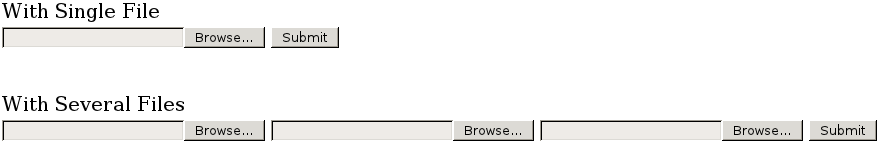
\includegraphics[width=15cm]{files}
\end{center}

SMEWS needs doPostIn and doPostOut functions. The doPostIn function allows to receive data with help of the in function. Otherwise, doPostOut function is similar to doPost. Moreover, the content-types must be specified to define the file type, which will be accepted by the application (the possibles content-types are contained in the file tools/mimesListPost which can be modified). It is very important to understand that the function doPostIn will be called for each part of multipart request (each file) and the function doPostOut will be called only once at the end.

\subsubsection{First example with one file}
\lstset{language=C}
\begin{lstlisting}
/*
<generator>
	<handlers doPostOut="doPostOut" doPostIn="doPostIn"/>
	<content-types>
		<content-type type="text/plain"/>
	</content-types>
</generator>
*/

/* file structure */
struct file_t {
	char *filename;
	uint16_t size;
};

/* dopostin function to operate post data */
static char doPostIn(uint8_t content_type, uint8_t call_number, 
char *filename, void **post_data) {
	uint16_t i = 0;
	short value;

	/* no file */
	if(!filename)
		return 1;

	/* file already treat */
	if(*post_data)
		return 1;

	/* counting filename size */
	while(filename[i++] != '\0');
	
	/* allocating memory */
	struct file_t *file = mem_alloc(sizeof(struct file_t));
	if(!file)
		return 1;
	file->filename = mem_alloc(i * sizeof(char));
	if(!file->filename)
		return 1;

	/* copying filename */
	i = 0;
	do{
		file->filename[i] = filename[i];
	}while(filename[i++] != '\0');

	/* counting and saving characters */
	i = 0;
	while((value = in()) != -1)
		i++;
	file->size = i;

	/* saving adress memory in post data */
	*post_data = file;

	return 1;
}

static char doPostOut(uint8_t content_type, void *data) {
	uint16_t i;
	if(data){
		/* printing data */
		out_str("The file \"");
		out_str(((struct file_t*)data)->filename);
		out_str("\" contains ");
		out_uint(((struct file_t*)data)->size);
		out_str(" characters.");

		/* counting filename size */
		i = 0;
		while(((struct file_t*)data)->filename[i++] != '\0');

		/* cleaning memory */
		mem_free(((struct file_t*)data)->filename,i * sizeof(char));
		mem_free(data,sizeof(struct file_t));
	}
	else
		out_str("No data file");
	return 1;
}
\end{lstlisting}

The doPostIn function has 4 parameters :
\begin{itemize}
\item \verb+ uint8_t content_type+ : the number of the content-type that have been parse by Smews. His number signification is available in the file core/defines.h after the compilation of SMEWS. 
\item \verb+uint8_t part_number+ : number of actual part with multipart data (0 if one part).
\item \verb+char *filename+ : filename of current file.
\item \verb+void **post_data+ : data flowing between dopostin and dopostout functions.
\end{itemize}

The doPostOut function has 2 parameters and they are similar to parameters of doPostIn function.
In the XML, the content-types tag must be specified, but can be empty. In this case, all types accepted in the tools/mimesListPost can be receive by the application.
\newline
Warning : the application must manage the allocation and freeing memory of {\tt post\_data}. Moreover, if the user want to use {\tt filename}, he must copy it and must not forget to free after use.  

\subsubsection{Second example with several files}
\lstset{language=C}
\begin{lstlisting}
/*
<generator>
	<handlers doPostOut="doPostOut" doPostIn="doPostIn"/>
	<content-types>
		<content-type type="text/plain"/>
	</content-types>
</generator>
*/

/* file structure */
struct file_t {
	char *filename;
	uint16_t size;
};

/* dopostin function to operate post data */
static char doPostIn(uint8_t content_type, uint8_t part_number, 
char *filename, void **post_data) {
	uint16_t i = 0;
	short value;

	/* no file */
	if(!filename)
		return 1;

	/* too many files (only 3 managed) */
	if(part_number > 2)
		return 1;

	/* allocating files structure if necessary */
	if(!*post_data) /*post_data used like tab*/
		*post_data = mem_alloc(3 * sizeof(struct file_t));
	if(!*post_data)
		return 1;

	/* counting filename size */
	while(filename[i++] != '\0');
	
	/* allocating filename memory */
	((struct file_t *)*post_data)[part_number].filename = mem_alloc(i * sizeof(char));
	if(!((struct file_t *)*post_data)[part_number].filename)
		return 1;

	/* copying filename */
	i = 0;
	do{
		((struct file_t *)*post_data)[part_number].filename[i] = filename[i];
	}while(filename[i++] != '\0');

	/* counting and saving characters */
	i = 0;
	while((value = in()) != -1)
		i++;
	((struct file_t *)*post_data)[part_number].size = i;

	return 1;
}

static char doPostOut(uint8_t content_type, void *post_data){
	if(post_data){
		uint8_t j;
		for(j = 0 ; j < 3 ; j++){
			if(!((struct file_t *)post_data)[j].filename)
				continue;
			uint8_t i;
			/* printing data */
			out_str("\nThe file \"");
			out_str(((struct file_t *)post_data)[j].filename);
			out_str("\" contains ");
			out_uint(((struct file_t *)post_data)[j].size);
			out_str(" characters.");
			/* cleaning filename */
			i = 0;
			while(((struct file_t *)post_data)[j].filename[i++] != '\0');
			mem_free(((struct file_t *)post_data)[j].filename,i * sizeof(char));
		}
		/* cleaning tab */
		mem_free(post_data,3 * sizeof(struct file_t));
	}
	else
		out_str("No data file");
	return 1;
}
\end{lstlisting}
This example uses {\tt part\_number} to manipulate several files and data are saved in a tab, pointed by post\_data.

Note : multipart is necessary if you use HTML form. But if you construct packets, Smews is able to process them (for example, text/plain like content-type and all data in request post data).

\section{Web Application SConscript}

Every Web application can provide a customized SConscript file, giving specific instruction for the pre-compilation phase. For a good example take a look in the \texttt{apps/welcome} folder, containing such a script. Here, we only detail the most interesting part of this file:
\lstset{language=python}
\begin{lstlisting}
[...]
appListName = 'appList.js'
appListPath = os.path.join(genDir,tmpBase,appListName)
appListAbsPath = os.path.join(sconsBasePath,appListPath)

appList = open(appListAbsPath,'w')
if len(dirsMap.keys()) > 2:
    appList.write('var appList = new Array();\n')
    appsCount = 0
    for dir in dirsMap.keys():
        if dir != 'welcome' and dir != httpCodesDir:
                 [.. Code Missing ..] # Get Web Content Files
                 [.. Code Missing ..] # Write line in .js
    # write title or empty string
    if appsCount > 0:
        appList.write('var appTitle = \"' + target.capitalize() + '
app examples:\";\n')
    else:
        appList.write('var appTitle = \"\";\n')
else:
    appList.write('var appTitle = \"\";\n')
appList.close()

ret = {appListPath: os.path.join(dirsMap['smews'],appListName)}
Return('ret')
\end{lstlisting}

The above lines iterate over the dirsMap hash map which has been built by the main Smews SCons files. It contains the set of applications being compiled with Smews (to be more precise, a set of associations between application names and paths). This code creates a \verb+appList.js+ file with code for adding links to the main page of the \verb+welcome+ application, links which point to other applications that were also compiled along with it. The generated \verb+applist.js+ file is embedded in \verb+index.html+ of the \verb+welcome+ application and then referenced when needed to display link to applications:
\lstset{language=html}
\begin{lstlisting}
[...]
<script type="text/javascript" src="appList.js"> </script>
[...]
\end{lstlisting}


\section{Synthesis of the features}

We give here an synthetic and exhaustive list of the features available when writing a dynamic content generator for Smews:

\begin{itemize}
\item \rtab{appsxml} details the XML markers available for sue in comment of C the files that need to be considered as a Web resource and associated to an URL;
\item \rtab{appscallbacks} gives the list of the callbacks a dynamic Web resource can implement;
\item \rtab{appssyscalls} lists the functions provided by Smews that can be called in any Web applicative code.
\end{itemize}

\begin{table}[htb]
    \fbox{
      \colorbox{black!10}{
		\begin{minipage}{1\textwidth}
{\tt <generator />}
\begin{quote} root of the applicative meta-data \end{quote}

{\tt <handlers init="<funcName>" initGet="<funcName>" doGet="<funcName>" />}
\begin{quote} callback functions definition \end{quote}

{\tt <properties persistence="persistent|idempotent|volatile"\\
interaction="rest|alert|stream" channel="<channelNem>" />}
\begin{quote} defines the properties of the Web resource \end{quote}

{\tt <args />}
\begin{quote} defines the possible URL arguments (set of {\tt arg} markers) \end{quote}

{\tt <arg name="<str>" type="uint8|uint16|uint32|str" size="<nBytes>" />}
\begin{quote} defines one argument \end{quote}

{\tt <content-types />}
\begin{quote} defines the possible content-types \end{quote}

{\tt <content-type type="<str>"/>}
\begin{quote} defines one content-type \end{quote}
		\end{minipage}
      }
   } 
\caption{XML markers for dynamic contents}
\label{tab:appsxml}
\end{table}

\begin{table}[htb]
    \fbox{
      \colorbox{black!10}{
		\begin{minipage}{1\textwidth}
{\tt char (init\_app\_func\_t)(void)}
\begin{quote} initialization of the applications, returning 1 if ok, 0 if ko. \end{quote}

{\tt char (initget\_app\_func\_t)(struct args\_t *)}
\begin{quote} called as soon as a get request is received, returning 1 if ok, 0 if ko. The parameter targets the parsed URL arguments. \end{quote}

{\tt char (doget\_app\_func\_t)(struct args\_t *)}
\begin{quote} called when the HTTP response is ready to be sent, returning 1 if ok, 0 if ko. The parameter targets the parsed URL arguments. This function is in charge of generating the HTTP response {\it via} {\tt out\_*} calls. \end{quote}

{\tt char (generator\_dopost\_in\_func\_t)(uint8\_t,uint8\_t,char *,void **)}
\begin{quote} called when the HTTP request is ready to be processed, returning 1 if ok, 0 if ko. The parameter are the content-type, the number of part, the filename of current file and the post data. This function is in charge of collecting posta data of HTTP request {\it via} {\tt in} calls. \end{quote}

{\tt char (generator\_dopost\_out\_func\_t)(uint8\_t,void *)}
\begin{quote} called when the HTTP response is ready to be sent, returning 1 if ok, 0 if ko. The parameters are the content-type and the post data. This function is in charge of generating the HTTP response {\it via} {\tt out\_*} calls. \end{quote}

	\end{minipage}
 	}
 } 
\caption{Functions handlers provided by Web applications}
\label{tab:appscallbacks}
\end{table}

\begin{table}[htb]
    \fbox{
      \colorbox{black!10}{
		\begin{minipage}{1\textwidth}
{\tt out\_c(char c)}
\begin{quote} to be used in the {\tt doGet} callback, thus adding the {\tt c} byte to the HTTP response that is currently generated \end{quote}

{\tt out\_uint(uint16\_t i)}
\begin{quote} to be used in the {\tt doGet} callback, thus adding the {\tt i} integer to the HTTP response that is currently generated \end{quote}

{\tt out\_str(const char str[])}
\begin{quote} to be used in the {\tt doGet} callback, thus adding the {\tt str} string to the HTTP response that is currently generated \end{quote}

{\tt short in()}
\begin{quote} to be used in the {\tt doPostIn} callback, thus receiving post data \end{quote}

{\tt trigger\_channel(const struct output\_handler\_t *handler)}
\begin{quote} usable in any function, it triggers a Comet channel, useful for alert or stream interaction modes \end{quote}

{\tt set\_timer(timer\_func\_t callback, uint16\_t period\_millis)}
\begin{quote} usable in any function, it allows to automatically call the {\tt callback} function every {\tt period\_millis} milliseconds \end{quote}
		\end{minipage}
      }
   } 
\caption{Functions provided by Smews}
\label{tab:appssyscalls}
\end{table}


\chapter{Creating an application for managing non-TCP packets}
\label{ch:gpip}

Smews now includes a feature called \textit{general purpose ip handler
  (GPIP)}. This features allows one to develop an application that will handle
non-TCP packets.

This new feature emerged from a discussion on how to correctly implement the
ICMPv6 Neighbor Solicitation packets to finish the IPv6 port on the mbed
ethernet target. It has been clear to us that handling those messages should
neither be in core nor in target specific code. Indeed, ICMPv6 should benefit
more than just a target and is outside smews main core (as smews core is
designed to handle HTTP). Thus, the decision was to implement a way for a
developper to add a Smews application that has 2 handler functions and
associate them to a IP protocol number (e.g. 1 for ICMPv4 or 58 for ICMPv6, 17
for UDP...). The functions are for processing input packets and generate an
output.

GPIP applications are standard smews applications that can define a new type of
generator. Thus, they can also integrates an associated web application,
although it is not mandatory. To illustrate this feature, this section will
describe an application for answering ICMPv4 echo request protocol.

\section{Declaring GPIP generators}
\label{sec:gpipgenerators}

As for a web dynamic application, a GPIP application consists in at least one
\textbf{.c} file with XML metadata to describe the application generator. The
metadata must declare two handlers and a protocol number.

The two handlers are called when a packet is received and when smews is ready
to generate a response. The XML metadata for our application will thus be:

\begin{lstlisting}
/*
<generator>
        <handlers doPacketIn="icmp4_packet_in" doPacketOut="icmp4_packet_out"/>
        <properties protocol="1" />
</generator>
 */
\end{lstlisting}

The \verb!doPacketIn! attribute declares the function that will be called by
smews when a packet is received. The \verb!doPacketOut! attribute declares the
function that will be called when smews is ready to generate an answer. In our
example, the handlers are the two C functions \verb!icmp4_packet_in! and
\verb!icmp4_packet_out!.

The protocol number is given by the \verb!protocol! property and is set to
1 which is the protocol number of ICMPv4. This value is the \textbf{Protocol}
field of an IPv4 packet and the \textbf{Next Header} field of an IPv6 packet.


\section{Handlers}
\label{sec:handlers}

The prototype of the handler functions is as follows:

\begin{lstlisting}
  char handler_func(const void *connection);
\end{lstlisting}

The \verb!connection! parameter is a handle that will allow the developer to
get some information on the incoming packet such as its remote IP address, its
payload size... 

\subsection{Packet information}
\label{sec:packetattributes}

To get information on an incoming packet, the application can use the following
functions. All the functions take the connection handle as parameter.

\begin{enumerate}
\item \verb!get_local_ip!~: returns the ip to which the packet was sent. Yet,
  smews has only one IP address so it returns the IP that was defined at
  compile time, but a smews version that can have multiple local IP (for
  example with multiple interfaces) may be developed later,
\item \verb!get_remote_ip!~: returns the ip from which the packet was sent,
\item \verb!get_payload_size!~: returns the payload size of the packet (it does not include IP header size),
\item \verb!get_protocol!~: returns the protocol that triggered the call to
  this functions. It allows one to have the same handler for multiple protocols
\item \verb!get_send_code!~: to be used in the \texttt{doPacketOut}
  handler. This returns the return value of the corresponding
  \texttt{doPacketIn} function. This is needed because due to the smews
  scheduler, the \texttt{doPacketOut} is not guaranteed to be called right
  after the \texttt{doPacketIn} that triggered it.
\end{enumerate}

\subsection{\texttt{doPacketIn} handler}
\label{sec:dopacketin}


The handler is called when a packet with the corresponding protocol number is
received by smews. After decoding the IP header, smews called the
\texttt{doPacketIn} handler. The handler can then call the \verb!in()! function
to get the content of the packet, byte per byte.

The function must return 0 if \textbf{no} reply has to be generated. Thus, in
the \texttt{doPacketIn} function returns 0, then the \texttt{doPacketOut} will
\textbf{not} be called.

If an answer needs to be generated, the function can return any non-zero
value. It will be possible to get this return value back when generating the
reply is generated in the \texttt{doPacketOut} function use the
\verb!get_send_code()! function.

Here is a sample code that interprets an ICMPv4 echo request packet (the
\verb!checksum_*! functions are provided by smews)~:

\begin{lstlisting}
char icmp4_packet_in(const void *connection_info)
{
	uint8_t tmp;
	uint16_t payload_size = get_payload_size(connection_info);
	int i;

	checksum_init();
	tmp = in(); /* type */

	if (tmp != ICMP_ECHO_REQUEST)
		return 0; /* drop packet and do not generate a reply */
	checksum_add(tmp);
	tmp = in(); /* code */
	checksum_add(tmp);

	checksum[S0] = in();
	checksum[S1] = in();
	checksum_add16(UI16(checksum));

	identifier[S0] = in();
	identifier[S1] = in();
	checksum_add16(UI16(identifier));

	sequence_number[S0] = in();
	sequence_number[S1] = in();
	checksum_add16(UI16(sequence_number));
	for (i = 0 ; i < payload_size - ICMP_HEADER_SIZE; ++i)
	{
		icmp_payload[i] = in();
		checksum_add(icmp_payload[i]);
	}
	buffer_size = payload_size - ICMP_HEADER_SIZE;
	checksum_end();
	if(UI16(current_checksum) != 0xffff)
		return 0; /* invalid checksum */
	return 1;
}
\end{lstlisting}


\subsection{\texttt{doPacketOut} handler}
\label{sec:dopacketout}

This handler is called by Smews when it is ready to generate a reply. This
function is quite similar to a \texttt{doGet} handler. It simply generate the
response packet, byte per byte, using the \verb!out_c()! function. 

In the \texttt{doPacketOut}, the \verb!get_*! functions described earlier can
still be called to get information on the incoming packet that triggered the
reply. Here is an example that implements the ICMPv4 reply associated to the
previously described request~:

\begin{lstlisting}
char icmp4_packet_out(const void *connection_info)
{
	int i;
	/* generate reply */

	out_c(ICMP_ECHO_REPLY); /* type */
	out_c(0);  /* code */

	/* Generate checksum from request one, only the type byte has change,
	 * so the value can be reused to accelerate the computation of the checksum
	 */
	UI16(checksum) += (ICMP_ECHO_REQUEST << 8);
	if ((UI16(checksum) >> 8) < ICMP_ECHO_REQUEST) /* overflow, should add one */
		UI16(checksum)++;
	out_c(checksum[S0]);
	out_c(checksum[S1]);
	out_c(identifier[S0]);
	out_c(identifier[S1]);
	out_c(sequence_number[S0]);
	out_c(sequence_number[S1]);
	for (i = 0 ; i < buffer_size ; ++i)
	{
		out_c(icmp_payload[i]);
	}
	return 0;
}
\end{lstlisting}


\section{Synthesis of the features}

We give here an synthetic and exhaustive list of the features available when writing a GPIP generator in Smews:

\begin{itemize}
\item \rtab{gpip-appsxml} details the XML markers available for sue in comment of C the files that need to be considered as a GPIP generator,
\item \rtab{gpip-appscallbacks} gives the list of the callbacks a GPIP generator can implement,
\item \rtab{gpip-appssyscalls} lists the functions provided by Smews that can be called in any GPIP application.
\end{itemize}

\begin{table}[htb]
    \fbox{
      \colorbox{black!10}{
		\begin{minipage}{1\textwidth}
{\tt <generator />}
\begin{quote} root of the applicative meta-data \end{quote}

{\tt <handlers init="<funcName>" doPacketIn="<funcName>" doPacketOut="<funcName>" />}
\begin{quote} callback functions definition \end{quote}

{\tt <properties protocol="<protocolNumber>" />}
\begin{quote} defines the protocol number associated to the GPIP generator \end{quote}
\end{minipage}
}
} 
\caption{XML markers for GPIP application}
\label{tab:gpip-appsxml}
\end{table}

\begin{table}[htb]
    \fbox{
      \colorbox{black!10}{
		\begin{minipage}{1\textwidth}
{\tt char (init\_app\_func\_t)(void)}
\begin{quote} initialization of the applications, returning 1 if ok, 0 if ko. \end{quote}

{\tt char (do\_packet\_in\_func\_t)(struct args\_t *)}
\begin{quote} called as soon as a packet is received, returning non zero value if the \texttt{doPacketOut} callback has to be called.\end{quote}

{\tt char (do\_packet\_out\_func\_t)(struct args\_t *)}
\begin{quote} called when the response is ready to be sent. This function is in charge of generating the response {\it via} {\tt out\_c} calls. \end{quote}

	\end{minipage}
 	}
 } 
\caption{Functions handlers provided by GPIP applications}
\label{tab:gpip-appscallbacks}
\end{table}

\begin{table}[htb]
    \fbox{
      \colorbox{black!10}{
		\begin{minipage}{1\textwidth}
{\tt out\_c(char c)}
\begin{quote} to be used in the {\tt doPacketOut} callback, thus adding the {\tt c} byte to the response that is currently generated \end{quote}

{\tt short in()}
\begin{quote} to be used in the {\tt doPacketIn} callback, thus receiving packet data \end{quote}

{\tt unsigned char *get\_local\_ip(const void *connection, unsigned char *ip)}
\begin{quote} Gets the local ip associated to a packet. Can be called in \texttt{doPacketIn} and \texttt{doPacketOut}. \end{quote}

{\tt unsigned char *get\_remote\_ip(const void *connection, unsigned char *ip)}
\begin{quote} Gets the remote ip associated to a packet. Can be called in \texttt{doPacketIn} and \texttt{doPacketOut}. \end{quote}

{\tt unsigned char *get\_payload\_size(const void *connection)}
\begin{quote} Gets size of the packet (without IP header). Can be called in \texttt{doPacketIn} and \texttt{doPacketOut}. \end{quote}

{\tt unsigned char *get\_send\_code(const void *connection)}
\begin{quote} Gets the return value of the \texttt{doPacketIn} callback. Can be called in \texttt{doPacketOut}. \end{quote}

		\end{minipage}
      }
   } 
\caption{Functions provided by Smews}
\label{tab:gpip-appssyscalls}
\end{table}


\chapter{Credits}

\section{Contributors}

\begin{description}
 \item[Simon Duquennoy] is the main author of Smews
 \item[Thomas So\"{e}te] wrote the WSN430 port and the MBED SLIP port
 \item[Geoffroy Cogniaux] wrote the FunCard7 port
 \item[Alex Negrea] is the main author of this user guide and wrote the TLS
implementation (only available in the svn repos)
 \item[Geoffrey Chavepeyer \textnormal{and} Fabien Duchêne] implemented the IPv6
support
\item[Emilien Hidden \textnormal{and} Olivier Szika] implemented the support
  for POST requests
 \item[Thomas Vantroys] wrote the Arduino port
 \item[Michaël Hauspie] wrote the MBED ethernet port, the GPIP feature and the
   ICMPv4 and ICMPv6 applications
 \item[Jean-Fran\c{c}ois Hren] designed the Smew (bird) in the Smews logo ;)
\end{description}
Thanks to \textbf{Gilles Grimaud} for his kind supervision and his wise advices.

\section{License}

Smews is under CeCILL license (\url{http://www.cecill.info/}) compliant with the GPL licence of SOSSE and TUN-TAP. It also includes part of the softwares listed below:
\begin{itemize}
 \item SOSSE: Matthias Br\"{u}stle -- http://www.mbsks.franken.de/sosse/
 \item TUN-TAP: Maxim Krasnyansky -- http://vtun.sourceforge.net/tun/
\end{itemize}

\end{document}
